\chapter{离子与离子溶液}\label{ch:g9:ions}

健身房长椅上放着两杯澄清的饮料：一瓶运动饮料，
标榜含有“电解质”；另一杯是加糖的水。在实验室里，两块
金属极板分别接上电池和一只小灯泡，依次浸入两种液体中。
在运动饮料中灯泡亮起；在加糖的水中灯泡保持暗淡。
第一种液体中有某种物质能够携带电荷，糖却不能，
这种物质就是\omterm{def:g9:ions:ion}{离子}。

\begin{recall}
\omterm{def:g7:atoms-and-molecules:atom}{原子}含有\omterm{def:g9:inside-the-atom:nucleus}{原子核}，核中有 $Z$ 个\omterm{def:g9:inside-the-atom:proton}{质子}，每个\omterm{def:g9:inside-the-atom:proton}{质子}带电 $+e$，
核外有 $Z$ 个\omterm{def:g9:inside-the-atom:nucleus}{电子}，每个\omterm{def:g9:inside-the-atom:nucleus}{电子}带电 $-e$：\omterm{def:g7:atoms-and-molecules:atom}{原子}呈电中性
（见\cref{ch:g9:inside-the-atom}）。溶于水的\omterm{def:g6:solutions-and-solubility:solute}{溶质}可形成
\omterm{def:g6:solutions-and-solubility:solute}{水溶液}（见\cref{ch:g6:solutions-and-solubility}）。\omterm{def:g7:identifying-substances:characteristic-test}{特征检验}
通过可见的结果检出某种物质
（见\cref{ch:g7:identifying-substances}）。
\end{recall}

\begin{omfigure}
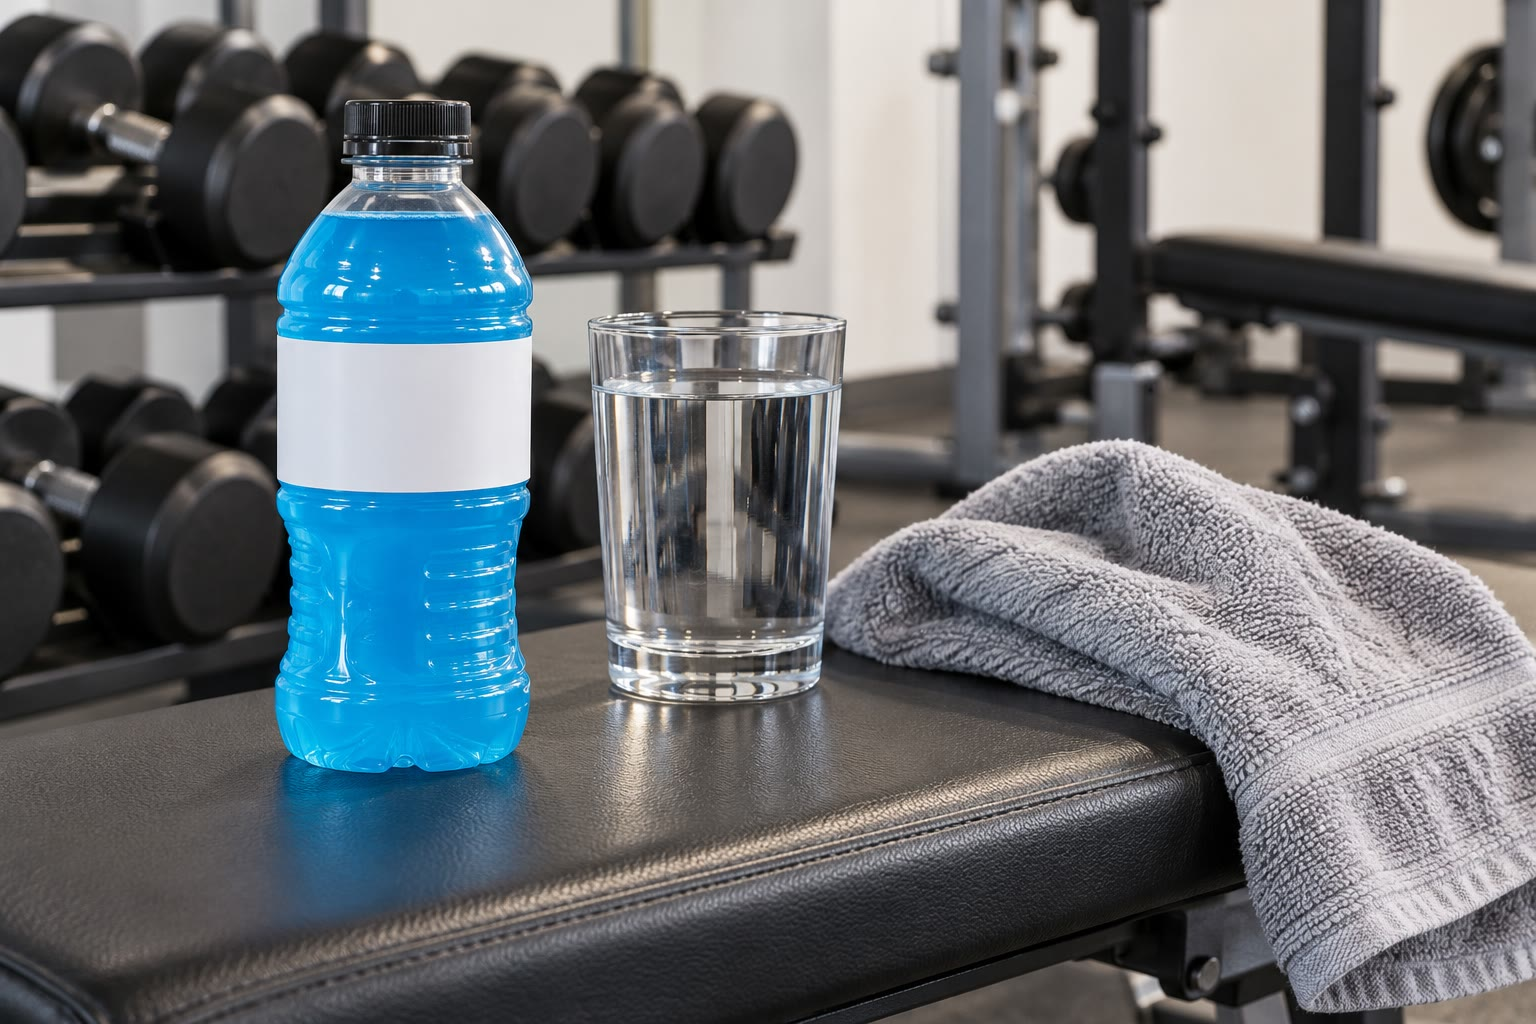
\includegraphics[width=0.5\linewidth]{images/book1/ai/g9-sports-drink.jpg}

{\small 一瓶运动饮料和一杯水：饮料中含有
\omterm{def:g2:mixing-and-dissolving:dissolve}{溶解}的\omterm{def:g9:ions:ion}{离子}。}
\end{omfigure}

\section{得失电子的原子}

\begin{definition}[离子、阳离子、阴离子]\label{def:g9:ions:ion}
称\emph{离子}\index{离子}为失去或
得到一个或多个\omterm{def:g9:inside-the-atom:nucleus}{电子}、因而带电荷的\omterm{def:g7:atoms-and-molecules:atom}{原子}或\omterm{def:g7:atoms-and-molecules:atom}{原子}团。
带正电荷、失去\omterm{def:g9:inside-the-atom:nucleus}{电子}的离子称为
\emph{阳离子}\index{阳离子}；带负电荷、得到\omterm{def:g9:inside-the-atom:nucleus}{电子}的离子称为
\emph{阴离子}\index{阴离子}。电荷写在化学式的右上角：
\ce{Na+}、\ce{Cu^{2+}}、\ce{Cl-}。
\end{definition}

\begin{example}[钠和氯]\label{ex:g9:ions:na-cl}
一个钠\omterm{def:g7:atoms-and-molecules:atom}{原子}含 11 个\omterm{def:g9:inside-the-atom:proton}{质子}和 11 个\omterm{def:g9:inside-the-atom:nucleus}{电子}，失去一个\omterm{def:g9:inside-the-atom:nucleus}{电子}后
变为钠\omterm{def:g9:ions:ion}{离子} \ce{Na+}，含 11 个\omterm{def:g9:inside-the-atom:proton}{质子}和 10 个\omterm{def:g9:inside-the-atom:nucleus}{电子}，电荷为
$+1$：
\[
  \ce{Na -> Na+ + e-}.
\]
一个氯\omterm{def:g7:atoms-and-molecules:atom}{原子}含 17 个\omterm{def:g9:inside-the-atom:proton}{质子}和 17 个\omterm{def:g9:inside-the-atom:nucleus}{电子}，得到一个\omterm{def:g9:inside-the-atom:nucleus}{电子}后
变为氯\omterm{def:g9:ions:ion}{离子} \ce{Cl-}，含 17 个\omterm{def:g9:inside-the-atom:proton}{质子}和 18 个\omterm{def:g9:inside-the-atom:nucleus}{电子}：
\[
  \ce{Cl + e- -> Cl-}.
\]
\end{example}

\begin{omfigure}
\begin{tikzpicture}[font=\small]
  \foreach \x/\name/\p/\e/\ch/\col in {0/{钠原子}/11/11/0/omDef,
      3.7/{钠离子 \ce{Na+}}/11/10/+1/omProp,
      8.0/{氯原子}/17/17/0/omDef, 11.7/{氯离子 \ce{Cl-}}/17/18/$-1$/omProp} {
    \node[draw=\col, fill=\col!6, rounded corners=2pt, align=center, text width=2.4cm]
      at (\x,0) {\textbf{\name}\\ \p\ 个质子 \\ \e\ 个电子 \\ 电荷 \ch};
  }
  \draw[->, thick, omProp] (1.45,0) -- (2.25,0) node[midway, above, text=black,
    font=\footnotesize, align=center] {失去 \\ 1 \ce{e-}};
  \draw[->, thick, omProp] (9.45,0) -- (10.25,0) node[midway, above, text=black,
    font=\footnotesize, align=center] {得到 \\ 1 \ce{e-}};
\end{tikzpicture}

{\small 钠\omterm{def:g7:atoms-and-molecules:atom}{原子}失去一个\omterm{def:g9:inside-the-atom:nucleus}{电子}变为钠\omterm{def:g9:ions:ion}{离子}；
氯\omterm{def:g7:atoms-and-molecules:atom}{原子}得到一个\omterm{def:g9:inside-the-atom:nucleus}{电子}变为氯\omterm{def:g9:ions:ion}{离子}。\omterm{def:g9:inside-the-atom:proton}{质子}数
不变。}
\end{omfigure}

\begin{proposition}[一些常见的离子]\label{prop:g9:ions:common}
单\omterm{def:g7:atoms-and-molecules:atom}{原子}\omterm{def:g9:ions:ion}{离子}由一个\omterm{def:g7:atoms-and-molecules:atom}{原子}构成，多\omterm{def:g7:atoms-and-molecules:atom}{原子}\omterm{def:g9:ions:ion}{离子}由一组
始终结合在一起的\omterm{def:g7:atoms-and-molecules:atom}{原子}构成：
\begin{center}
\small
\begin{tabular}{llll}
\hline
\omterm{def:g9:ions:ion}{阳离子} & & \omterm{def:g9:ions:ion}{阴离子} & \\
\hline
钠\omterm{def:g9:ions:ion}{离子} & \ce{Na+} & 氯\omterm{def:g9:ions:ion}{离子} & \ce{Cl-} \\
钾\omterm{def:g9:ions:ion}{离子} & \ce{K+} & 氢氧根\omterm{def:g9:ions:ion}{离子} & \ce{OH-} \\
钙\omterm{def:g9:ions:ion}{离子} & \ce{Ca^{2+}} & 硝酸根\omterm{def:g9:ions:ion}{离子} & \ce{NO3-} \\
镁\omterm{def:g9:ions:ion}{离子} & \ce{Mg^{2+}} & 碳酸根\omterm{def:g9:ions:ion}{离子} & \ce{CO3^{2-}} \\
铜(II)\omterm{def:g9:ions:ion}{离子} & \ce{Cu^{2+}} & 硫酸根\omterm{def:g9:ions:ion}{离子} & \ce{SO4^{2-}} \\
铁(II)、铁(III)\omterm{def:g9:ions:ion}{离子} & \ce{Fe^{2+}}, \ce{Fe^{3+}} & & \\
锌\omterm{def:g9:ions:ion}{离子} & \ce{Zn^{2+}} & & \\
铝\omterm{def:g9:ions:ion}{离子} & \ce{Al^{3+}} & & \\
铵根\omterm{def:g9:ions:ion}{离子} & \ce{NH4+} & & \\
\hline
\end{tabular}
\end{center}
\end{proposition}

\section{离子化合物及其化学式}

\begin{definition}[离子化合物]\label{def:g9:ions:ionic-compound}
称\emph{离子化合物}\index{离子化合物}为由\omterm{def:g9:ions:ion}{阳离子}和\omterm{def:g9:ions:ion}{阴离子}
按适当比例组成、使整体不带电荷的化合物。其化学式
给出\omterm{def:g9:ions:ion}{离子}的个数比，但不标电荷：\ce{NaCl} 表示氯化钠，
即一个 \ce{Na+} 对应一个 \ce{Cl-}；\ce{CaCl2} 表示氯化钙，
两个 \ce{Cl-} 对应一个 \ce{Ca^{2+}}。
\end{definition}

\begin{method}[写出离子化合物的化学式]\label{met:g9:ions:formula}
\begin{enumerate}
  \item 写出两种\omterm{def:g9:ions:ion}{离子}及其电荷，\omterm{def:g9:ions:ion}{阳离子}在前。
  \item 找出各\omterm{def:g9:ions:ion}{离子}的最少个数，使
        总电荷为零。
  \item 将这些个数写作\omterm{def:g7:atoms-and-molecules:formula}{下标}；若多\omterm{def:g7:atoms-and-molecules:atom}{原子}\omterm{def:g9:ions:ion}{离子}需要\omterm{def:g7:atoms-and-molecules:formula}{下标}，
        则应加括号。
\end{enumerate}
氧化铝：\ce{Al^{3+}} 和 \ce{O^{2-}}；$2 \times (+3) + 3 \times
(-2) = 0$，故为 \ce{Al2O3}。氢氧化铁(III)：\ce{Fe^{3+}} 和三个
\ce{OH-}：\ce{Fe(OH)3}。
\end{method}

\begin{proposition}[离子固体是离子的堆叠]\label{prop:g9:ions:solid}
在食盐晶体中，钠\omterm{def:g9:ions:ion}{离子}与氯\omterm{def:g9:ions:ion}{离子}交替排列成
规则的三维堆叠，每个\omterm{def:g9:ions:ion}{离子}都被电荷相反的
\omterm{def:g9:ions:ion}{离子}包围，靠这些\omterm{def:g9:ions:ion}{离子}将其固定。一粒食盐含有
数以亿亿计的\omterm{def:g9:ions:ion}{离子}，其立方体外形反映了立方堆叠的结构。
\end{proposition}

\begin{omfigure}
\begin{minipage}[b]{0.5\linewidth}\centering
\begin{tikzpicture}[font=\small]
  \foreach \i in {0,...,5} \foreach \j in {0,...,4} {
    \pgfmathtruncatemacro\pp{mod(\i+\j,2)}
    \ifnum\pp=0 \node[aNa, minimum size=5mm] at (0.62*\i,0.62*\j) {};
    \else \node[aCl, minimum size=7.4mm] at (0.62*\i,0.62*\j) {};\fi
  }
\end{tikzpicture}

{\small 食盐晶体的一层：钠\omterm{def:g9:ions:ion}{离子}（紫色，较小）与
氯\omterm{def:g9:ions:ion}{离子}（绿色）交替排列。}
\end{minipage}\hfill
\begin{minipage}[b]{0.3\linewidth}\centering
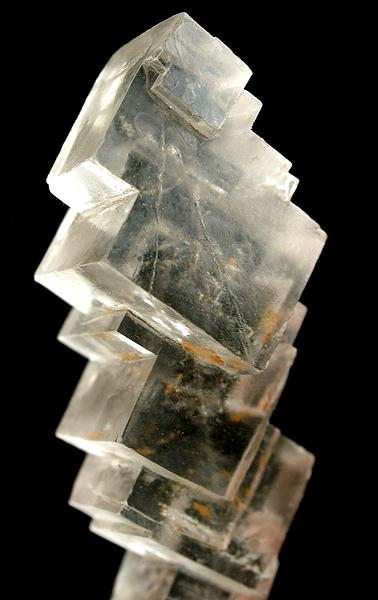
\includegraphics[height=4.6cm]{images/book1/halite.jpg}

{\small 石盐，天然岩盐。照片：Robert M.~Lavinsky，
CC BY-SA 3.0。}
\end{minipage}
\end{omfigure}

\section{离子溶液能导电}

\begin{notation}[状态符号 (aq)]\label{not:g9:ions:aq}
溶于水的\omterm{def:g9:ions:ion}{离子}或\omterm{def:g7:atoms-and-molecules:molecule}{分子}以 (aq) 标记，表示“\omterm{def:g6:solutions-and-solubility:solute}{水溶液}”：
\ce{Na+(aq)}, \ce{Cl-(aq)}.
\end{notation}

\begin{proposition}[离子溶液能导电]\label{prop:g9:ions:conduct}
\omterm{def:g9:ions:ionic-compound}{离子化合物}溶于水时，其\omterm{def:g9:ions:ion}{离子}分开，
并在溶液中自由移动：食盐水中含有 \ce{Na+(aq)} 和
\ce{Cl-(aq)}。移动的\omterm{def:g9:ions:ion}{离子}携带电荷，因此\omterm{def:g9:ions:ion}{离子}溶液
能导电。糖溶液中的\omterm{def:g7:atoms-and-molecules:molecule}{分子}不带电，
因而不导电；极纯的水也不导电。
\end{proposition}

\begin{inthelab}[哪些液体能导电？]
两块金属极板、一节低压电池和一个小灯泡由老师连接成
电路；极板依次浸入蒸馏水、
糖水、食盐水和硫酸铜溶液中，并在每次之间
冲洗。只有在两种\omterm{def:g9:ions:ion}{离子}溶液中，灯泡才会亮。
\end{inthelab}

\begin{omfigure}
\begin{tikzpicture}[font=\small, scale=1.1]
  \foreach \xs/\lit/\lab in {0/1/{盐水：灯泡发光}, 5.2/0/{糖水：灯泡不亮}} {
    \begin{scope}[xshift=\xs cm]
      \pic[transform shape] at (2,0) {beaker={0.7}{omWater!80}};
      \fill[black!45] (1.6,0.25) rectangle (1.7,2.6);
      \fill[black!45] (2.3,0.25) rectangle (2.4,2.6);
      \ifnum\lit=1 \fill[yellow!70, opacity=0.8] (3.4,3.0) circle (0.42);\fi
      \draw (1.65,2.6) -- (1.65,3.6) to[battery1] (3.4,3.6) -- (3.4,3.4)
        to[lamp] (3.4,2.6) -- (2.35,2.6);
      \node[anchor=north, align=center] at (2,-0.15) {\lab};
    \end{scope}
  }
\end{tikzpicture}

{\small 电导率测试：食盐水中，\omterm{def:g9:ions:ion}{离子}传导电流，
灯泡发亮；糖水中不含\omterm{def:g9:ions:ion}{离子}，灯泡
保持不亮。}
\end{omfigure}

\section{离子的沉淀检验}

\begin{definition}[沉淀]\label{def:g9:ions:precipitate}
两种溶液\omterm{def:g2:mixing-and-dissolving:mix}{混合}时，一种溶液中的\omterm{def:g9:ions:ion}{阳离子}与另一种溶液中的\omterm{def:g9:ions:ion}{阴离子}
可能结合成难溶的\omterm{def:g9:ions:ionic-compound}{离子化合物}。它呈细小的
固体，使液体变浑浊并\omterm{def:g3:separating-mixtures:decant}{沉降}，称为
\emph{沉淀}\index{沉淀}。这类反应称为
\emph{沉淀反应}\index{沉淀反应}。
\end{definition}

\begin{proposition}[常见离子的检验]\label{prop:g9:ions:tests}
滴入几滴\omterm{def:g7:identifying-substances:characteristic-test}{试剂}溶液，即可根据
所生成\omterm{def:g9:ions:precipitate}{沉淀}的颜色鉴定\omterm{def:g9:ions:ion}{离子}：
\begin{center}
\small
\begin{tabular}{llll}
\hline
待检\omterm{def:g9:ions:ion}{离子} & \omterm{def:g7:identifying-substances:characteristic-test}{试剂} & \omterm{def:g9:ions:precipitate}{沉淀} & 颜色 \\
\hline
铜（II） \ce{Cu^{2+}} & 氢氧化钠 & \ce{Cu(OH)2} & 蓝色 \\
铁（II） \ce{Fe^{2+}} & 氢氧化钠 & \ce{Fe(OH)2} & 绿色 \\
铁（III） \ce{Fe^{3+}} & 氢氧化钠 & \ce{Fe(OH)3} & 橙棕色 \\
锌 \ce{Zn^{2+}} & 氢氧化钠 & \ce{Zn(OH)2} & 白色 \\
铝 \ce{Al^{3+}} & 氢氧化钠 & \ce{Al(OH)3} & 白色 \\
氯\omterm{def:g9:ions:ion}{离子} \ce{Cl-} & 硝酸银 & \ce{AgCl} & 白色，见光变暗 \\
\hline
\end{tabular}
\end{center}
\end{proposition}

\begin{example}[沉淀反应的写法]\label{ex:g9:ions:equation}
只写出生成固体的\omterm{def:g9:ions:ion}{离子}，其余\omterm{def:g9:ions:ion}{离子}仍以\omterm{def:g2:mixing-and-dissolving:dissolve}{溶解}态存在，
不参与反应：
\[
  \ce{Cu^{2+}(aq) + 2OH-(aq) -> Cu(OH)2(s)}, \qquad
  \ce{Ag+(aq) + Cl-(aq) -> AgCl(s)}.
\]
\end{example}

\begin{omfigure}
\begin{tikzpicture}[font=\small, scale=0.95]
  \foreach \k/\pc/\lab in {0/blue!60/{\ce{Cu^{2+}}：蓝色}, 1/green!45!black!70/{\ce{Fe^{2+}}：绿色},
      2/orange!70!brown/{\ce{Fe^{3+}}：橙 \\褐色}, 3/white!85!black/{\ce{Zn^{2+}}：白色},
      4/white!85!black/{\ce{Al^{3+}}：白色}, 5/white!80!black/{\ce{Cl-}：白色}} {
    \pic[transform shape] at (\k*2.3,0) {testtube={0.5}{omWater!60}};
    \pic[transform shape] at (\k*2.3,0) {testtube={0.14}{\pc}};
    \node[anchor=north, align=center, font=\footnotesize, text width=2cm] at (\k*2.3,-0.15) {\lab};
  }
\end{tikzpicture}

{\small 前五支试管中的\omterm{def:g9:ions:precipitate}{沉淀}由氢氧化钠生成，
最后一支试管中的\omterm{def:g9:ions:precipitate}{沉淀}由硝酸银生成。}
\end{omfigure}

\begin{safety}{\ghs[0.82cm]{GHS05}\ghs[0.82cm]{GHS07}}
% ledger: ghs:NaOH, ghs:AgNO3
氢氧化钠：会引起严重的皮肤灼伤和眼损伤，并可能
腐蚀金属（GHS05）；稀溶液对皮肤和眼睛有刺激性（GHS07）。
硝酸银是检验氯\omterm{def:g9:ions:ion}{离子}的
\omterm{def:g7:identifying-substances:characteristic-test}{试剂}，具有氧化性和腐蚀性，对水生生物毒性极大。
护目镜、手套；\omterm{def:g7:identifying-substances:characteristic-test}{试剂}由教师逐滴分取。
\end{safety}

\begin{method}[离子的检验]\label{met:g9:ions:test}
\begin{enumerate}
  \item 取少量待测溶液于试管中。
  \item 逐滴加入\omterm{def:g7:identifying-substances:characteristic-test}{试剂}。
  \item 观察\omterm{def:g9:ions:precipitate}{沉淀}的颜色，并与表格对照。
  \item 得出结论。注意，检验的是\omterm{def:g9:ions:ion}{离子}，而非
        化合物：氯化铁溶液
        同时通过 \ce{Fe^{3+}} 和 \ce{Cl-} 的检验。
\end{enumerate}
\end{method}

\section{练习}

\begin{exercise}[$\star$]\label{exo:g9:ions:1}
什么是\omterm{def:g9:ions:ion}{离子}？\omterm{def:g9:ions:ion}{阳离子}与\omterm{def:g9:ions:ion}{阴离子}有何区别？
\end{exercise}

\begin{exercise}[$\star$]\label{exo:g9:ions:2}
一个镁\omterm{def:g7:atoms-and-molecules:atom}{原子}（含 12 个\omterm{def:g9:inside-the-atom:proton}{质子}）失去两个\omterm{def:g9:inside-the-atom:nucleus}{电子}。写出所形成\omterm{def:g9:ions:ion}{离子}的
化学式，并给出其\omterm{def:g9:inside-the-atom:proton}{质子}数和\omterm{def:g9:inside-the-atom:nucleus}{电子}数。
\end{exercise}

\begin{exercise}[$\star$]\label{exo:g9:ions:3}
写出氯化钾、氯化镁和
氧化钙的化学式（氧\omterm{def:g9:ions:ion}{离子}：\ce{O^{2-}}）。
\end{exercise}

\begin{exercise}[$\star$]\label{exo:g9:ions:4}
为什么盐水能导电，而糖水不能？
\end{exercise}

\begin{exercise}[$\star\star$]\label{exo:g9:ions:5}
写出硫酸铜（II）、氯化铝和
碳酸钠的化学式。
\end{exercise}

\begin{exercise}[$\star\star$]\label{exo:g9:ions:6}
向某溶液中加入氢氧化钠，生成橙棕色\omterm{def:g9:ions:precipitate}{沉淀}。
该溶液中含有哪种\omterm{def:g9:ions:ion}{离子}？写出
\omterm{def:g9:ions:precipitate}{沉淀反应}的方程式。
\end{exercise}

\begin{exercise}[$\star\star$]\label{exo:g9:ions:7}
硫酸根\omterm{def:g9:ions:ion}{离子} \ce{SO4^{2-}} 比其\omterm{def:g9:inside-the-atom:proton}{质子}多带几个\omterm{def:g9:inside-the-atom:nucleus}{电子}？
硝酸根\omterm{def:g9:ions:ion}{离子} \ce{NO3-} 呢？
\end{exercise}

\begin{exercise}[$\star\star$]\label{exo:g9:ions:8}
某溶液与硝酸银反应生成白色\omterm{def:g9:ions:precipitate}{沉淀}，与氢氧化钠反应生成蓝色\omterm{def:g9:ions:precipitate}{沉淀}。
写出\omterm{def:g2:mixing-and-dissolving:dissolve}{溶解}的\omterm{def:g9:ions:ionic-compound}{离子化合物}的名称，并写出其
化学式。
\end{exercise}

\begin{exercise}[$\star\star$]\label{exo:g9:ions:9}
观察食盐晶体层的图示。该层中位于中间的\omterm{def:g9:ions:ion}{离子}
有几个带异号电荷的相邻\omterm{def:g9:ions:ion}{离子}，
均在该层之内？
\end{exercise}

\begin{exercise}[$\star\star$]\label{exo:g9:ions:10}
写出
由 \ce{Fe^{2+}} 与 \ce{OH-} \omterm{def:g9:ions:ion}{离子}生成氢氧化铁（II）\omterm{def:g9:ions:precipitate}{沉淀}的方程式。
\end{exercise}

\begin{exercise}[$\star\star\star$]\label{exo:g9:ions:11}
某白色粉末可能是氯化锌或氯化钠。将其溶于
水后，与氢氧化钠反应生成白色\omterm{def:g9:ions:precipitate}{沉淀}。它是哪一种？
写出反应方程式。
\end{exercise}

\begin{exercise}[$\star\star\star$]\label{exo:g9:ions:12}
在氯化钙晶体中，
与 1000 个钙\omterm{def:g9:ions:ion}{离子}对应的氯\omterm{def:g9:ions:ion}{离子}有多少个？并验证该晶体呈电中性。
\end{exercise}

\section{周末问题：生锈的水井}

\begin{problem}[{周末问题——农舍水槽中的橙色污渍，两项检验，
以及一升井水中的铁离子数目}]
\label{pb:g9:ions:1}
农舍水井的水会在水槽中留下橙色污渍。某实验室
收到一份样品。刚取出时，水是澄清的；加入氢氧化钠后
生成绿色\omterm{def:g9:ions:precipitate}{沉淀}，该\omterm{def:g9:ions:precipitate}{沉淀}在表面与\omterm{def:g4:air-a-mixture-of-gases:air}{空气}接触处
一小时内转为橙棕色。该实验室
测得每升水中以铁\omterm{def:g9:ions:ion}{离子}形式存在的铁为 \qty{0.30}{mg}。
取\omterm{def:g9:inside-the-atom:proton}{核子}质量为 \qty{1.67e-27}{kg}，
铁\omterm{def:g7:atoms-and-molecules:atom}{原子}含 56 个\omterm{def:g9:inside-the-atom:proton}{核子}。

\medskip
\noindent\textbf{第一部分——检验。}
\begin{enumerate}
  \item 绿色\omterm{def:g9:ions:precipitate}{沉淀}表明含有哪种\omterm{def:g9:ions:ion}{离子}？写出
        该\omterm{def:g9:ions:precipitate}{沉淀}的化学式。
  \item 橙棕色\omterm{def:g9:ions:precipitate}{沉淀}表明含有哪种\omterm{def:g9:ions:ion}{离子}？写出
        其化学式。
  \item 铁（II）\omterm{def:g9:ions:ion}{离子}与铁（III）\omterm{def:g9:ions:ion}{离子}相差一个\omterm{def:g9:inside-the-atom:nucleus}{电子}。
        哪一种含有的\omterm{def:g9:inside-the-atom:nucleus}{电子}更多？它们各含多少个\omterm{def:g9:inside-the-atom:nucleus}{电子}
        （铁：$Z = 26$）？
  \item 写出氢氧化铁（III）\omterm{def:g9:ions:precipitate}{沉淀}生成的方程式。
\end{enumerate}

\medskip
\noindent\textbf{第二部分——污渍。}
\begin{enumerate}[resume]
  \item 在水槽中，澄清的水会慢慢变浑浊并呈橙色。哪种
        \omterm{def:g9:ions:ion}{离子}是水从井中取出时所含的，哪种
        \omterm{def:g9:ions:ion}{离子}又是最终所含的？
  \item 写出由铁（III）\omterm{def:g9:ions:ion}{离子}与氢氧根\omterm{def:g9:ions:ion}{离子}
        形成的\omterm{def:g9:ions:ionic-compound}{离子化合物}的化学式，并验证其呈电中性。
  \item 水中的铁能否在水从井中流出时通过\omterm{def:g3:separating-mixtures:filter}{过滤}除去？
        水变为橙色之后呢？请说明理由。
  \item 含铁\omterm{def:g9:ions:ion}{离子}的水是\omterm{def:g6:pure-substances-and-mixtures:pure-substance}{纯净物}吗？是\omterm{def:g6:pure-substances-and-mixtures:homogeneous}{均相
        混合物}吗？
\end{enumerate}

\medskip
\noindent\textbf{第三部分——计算\omterm{def:g9:ions:ion}{离子}数目。}
\begin{enumerate}[resume]
  \item 计算一个铁\omterm{def:g7:atoms-and-molecules:atom}{原子}的质量，单位为千克。
  \item 将 \qty{0.30}{mg} 换算为千克。
  \item 为什么可以取铁\omterm{def:g9:ions:ion}{离子}的质量
        等于铁\omterm{def:g7:atoms-and-molecules:atom}{原子}的质量？
  \item 计算一升井水中铁\omterm{def:g9:ions:ion}{离子}的数目。
\end{enumerate}
\end{problem}
